\documentclass[11pt]{article}
\usepackage{amsmath, amssymb, amsfonts,  graphicx, enumerate, float, wrapfig, hyperref}
\usepackage[margin=0.5in]{geometry}
\graphicspath{{./}}
\newcommand*{\vs}{\vspace{1cm}}
\newcommand*{\next}{\noindent}
\newcommand*{\set}{\setcounter{equation}{0}}

\begin{document}

\title{Notes - 4.1 Antiderivatives and Indefinite Integration}
\author{Juan J. Moreno Santos}
\date{November 2023}

\maketitle

\section{Warm-up}
1. Let $y=x^2\cos x$. $\frac{dy}{dx}=$\\
Apply the product rule:
\[\frac{d}{dx}(f(x)g(x))=f'(x)g(x)+f(x)g'(x)\]
Therefore,
\begin{align}
    y'&=2x\cos x+x^2(-\sin x)\\
    &=2x\cos x-x^2\sin x
\end{align}

\vs
\next
2. If $y=\frac{\sin x}{\cos x}$, then $\frac{dy}{dx}=$
Remember the trigonometric identity:
\[\frac{\sin x}{\cos x}=\tan x\]
Therefore,
\[\frac{d}{dx}\left(\frac{\sin x}{\cos x}\right)=\frac{d}{dx}(\tan x)=\sec^2 x\]

\section{Reversing derivatives}
\begin{align}
    \set
    2x=\frac{d}{dx}(x^2)&=\int 2xdx=x^2+C\\
    6x=\frac{d}{dx}(3x^2)&=\int x^{-2/3}dx=3x^{1/3}+C\\
    x^{-2/3}=\frac{d}{dx}(3x^{1/3})&=\int xdx=\frac{1}{2}x^2+C\\
    \frac{5}{3}x^{2/3}=\frac{d}{dx}(x^{5/3})&=\int \frac{5}{3}x^{2/3}dx=x^{5/3}+C\\
    -\sin x=\frac{d}{dx}(\cos x)\\
    \sin x=\frac{d}{dx}(-\cos x)\therefore &\int \sin xdx=-\cos x+C
\end{align}

\section{Applying an integral:}
\begin{align}
    \set
    \int (3x^2+\frac{1}{2}x^2+4)dx\\
    =x^3+\frac{1}{6}x^3+4x+C
\end{align}

\section{The fundamental theorem of Calculus:}
\[y=\int f(x)dx=F(x)+C\]
Where
\begin{enumerate}
    \item $f$ is the integran.
    \item $dx$ is the variable of integration.
    \item $F$ is an antiderivative of $f(x)$.
    \item $C$ is the constant of integration.
\end{enumerate}
Note the capital $F$.\\
Integral is a synonym of antiderivative.
\section{Integrals inside a derivative:}
If $\int f(x)dx=F(x)+C$, then:
\[\frac{d}{dx}\left(\int f(x)dx\right)=f(x)\]
In conclusion, differentiation is the "inverse" of integration and vice versa.\\
\begin{flushleft}
    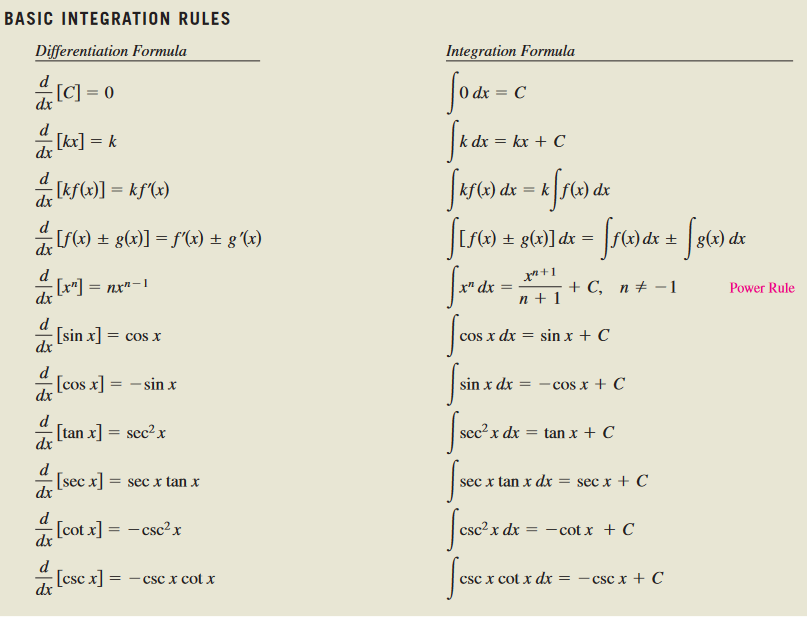
\includegraphics[scale=0.9]{Integration.png}
\end{flushleft}

\section{Warm-up 11/13/2023}
1. Let $y=\tan^2(3x)$. $\frac{dy}{dx}=$
\begin{align}
    \set
    \frac{dy}{dx}&=2(\tan(3x))\frac{d}{dx}(\tan(3x))\frac{d}{dx}(3x)\\
    &=2(\tan(3x))\sec^2(3x)\cdot3\\
    &=6(\tan(3x))\sec^2(3x)
\end{align}

2.\[\lim_{h\to0}\frac{\sin(\pi+h)-\sin(\pi)}{h}\]
\begin{align}
    \set
    &=\frac{d}{dx}(\sin(\pi))\\
    &=\cos(\pi)\\
    &=-1
\end{align}

\section{Triangular numbers}
\url{https://en.wikipedia.org/wiki/Triangular_number}\\
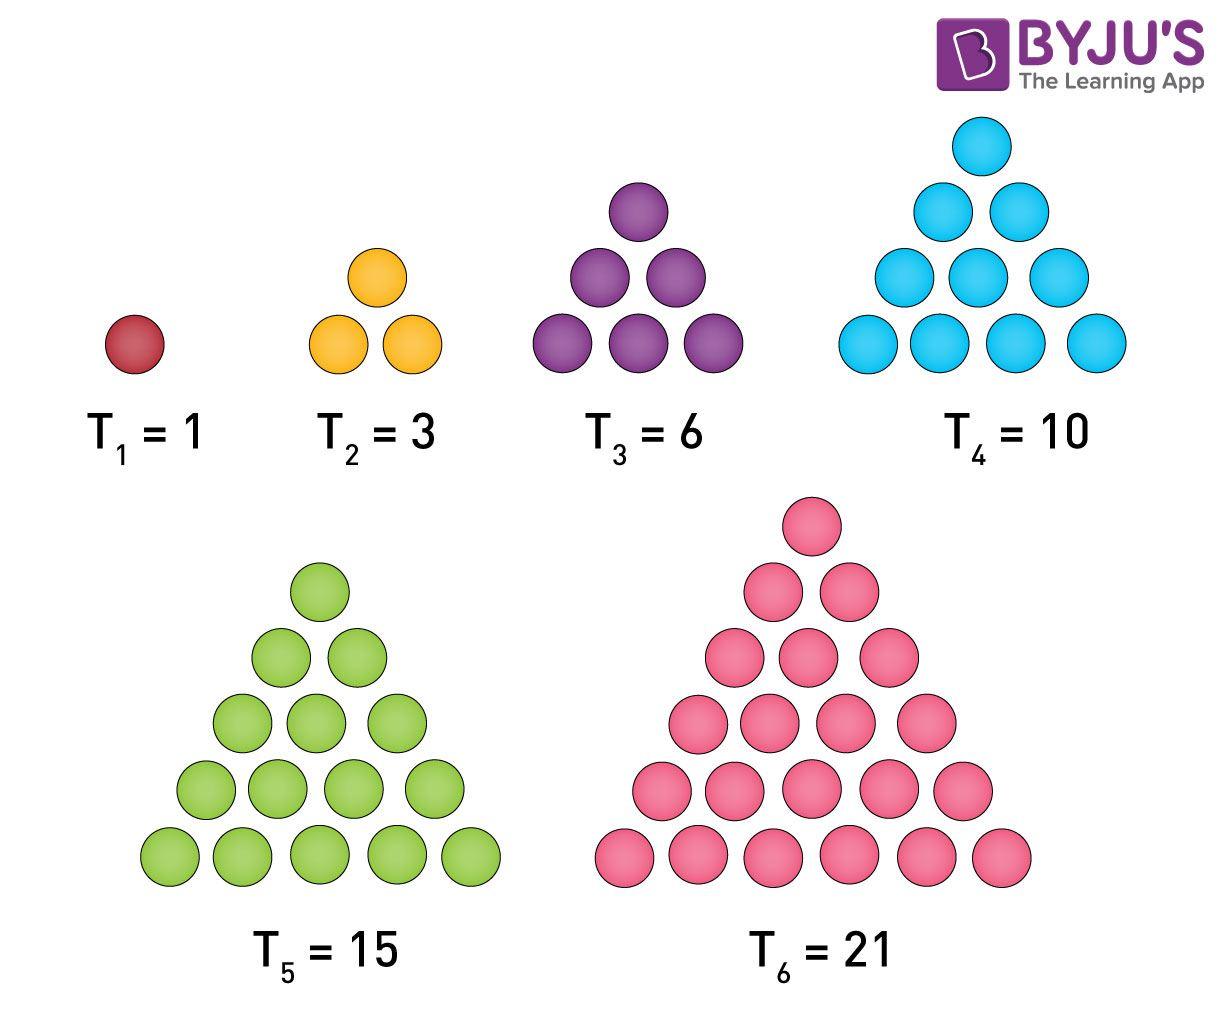
\includegraphics[scale=0.5]{triangular-numbers.jpg}
Triangular numbers are given by the following formulas:
\[\sum_{k=1}^{n}k=1+2+3+\cdots+n\]
\[\frac{n(n+1)}{2}\]
\[\frac{n^2+n}{2}\]
\[\left(\frac{n+1}{2}\right)\]
The first equation can be illustrated using a visual proof.[1] For every triangular number $T_{n}$, imagine a "half-rectangle" arrangement of objects corresponding to the triangular number, as in the figure below. Copying this arrangement and rotating it to create a rectangular figure doubles the number of objects, producing a rectangle with dimensions ${\displaystyle n\times (n+1)}$, which is also the number of objects in the rectangle. Clearly, the triangular number itself is always exactly half of the number of objects in such a figure, or: ${\displaystyle T_{n}={\frac {n(n+1)}{2}}}$. The example $T_4$ follows: 

\[2^{1/3}=\sqrt[3]{2}\approx 1.26\]
\[2^{-2/7}=\frac{1}{\sqrt[7]{(2)^2}}=\approx 0.82\]

\end{document}